\documentclass[12pt]{exam}
\usepackage[utf8]{inputenc}
%\usepackage[portuguese,brazil]{babel}
%\usepackage[margin=.75in]{geometry}
\usepackage{amsmath,amssymb}
\usepackage{multicol}
\usepackage{multirow}
\usepackage{float}
\usepackage{enumerate}
\usepackage{array}
\usepackage{graphicx}% delete the demo option in your actual code
\usepackage{xcolor}
\usepackage{tikz}

% \usepackage[usenames,dvipsnames]{pstricks}
\usepackage{epsfig}
\usepackage{pst-grad} % For gradients
\usepackage{pst-plot} % For axes
\usepackage[space]{grffile} % For spaces in paths
\usepackage{etoolbox} % For spaces in paths
% \makeatletter % For spaces in paths


\pointpoints{ponto}{pontos}
\hpword{Pontos:}
\vpword{Pontos}
\htword{Total}
\vtword{Total:}
\vsword{Resultado}


\SolutionEmphasis{\color{red}}
\CorrectChoiceEmphasis{\bf \color{red}}
\renewcommand{\solutiontitle}{\noindent\textbf{Solução:}\enspace}


\begin{document}

%Este exame contêm \numpages\ páginas (incluindo esta capa) e \numquestions\ questões.\\
%Total de \numpoints~ pontos.

%\begin{center}
%Grade Table (for teacher use only)\\
%\addpoints
%\gradetable[v][questions]
%\end{center}

%\noindent
%\rule[2ex]{\textwidth}{2pt}

\printanswers

\begin{center}
\textbf{{\Huge Atividades}}
\end{center}

\begin{questions}

\section*{Simplex}

\question Seja o Problema de Programação Linear a seguir:
	
	\begin{table}[H]
		\centering
			\begin{tabular}{c c c r c r c c }
			($PPL$) :&  Maximizar & $x_1$ & + & $x_2$   &  & &	\\
			& sujeito a: & $x_1$ & + & $4x_2$  & $\leq $ &	 4 \\
			 & & $3x_1$ & $+$ & $x_2$ &  = &	 1 \\
			 & & $x_1$ & , & $x_2$ &  $\geq$ &	 0
			\end{tabular}
	\end{table}	
	Resolva o PPL pelo método do simplex.
	
	\begin{solution}

	\begin{equation*}	
			\begin{array}{c r r c r c c c }
			(PPL) :& \text{Maximizar} & x_1  & + &  x_2    &  & &	\\
			           & \text{sujeito a:}  & x_1 & + & 4x_2  &  \leq  &	 4 \\
			           &                              & 3x_1 & + & x_2 &  = &	 1 \\
			           &                              & \multicolumn{6}{c}{x_1,~x_2 \geq 0}
			\end{array}	
	\end{equation*}
Adicionando variável de folga:
	\begin{equation*}	
			\begin{array}{c r r c r crc c c }
			(PPL) :& \text{Maximizar} & x_1   & + &  x_2   & + & 0x_3 &  & &	\\
			           & \text{sujeito a:}  & x_1   & + & 4x_2  & + &  x_3 &  =  &	 4 \\
			           &                              & 3x_1 & + & x_2    &     &        &  =  &	 1 \\
			           &                              & \multicolumn{6}{c}{x_1,~x_2,~x_3 \geq 0}
			\end{array}	
	\end{equation*}
	
	Criando o problema artificial (PA):
	\begin{equation*}	
			\begin{array}{c r r c r crcrc c c }
			(PA) :& \text{Minimizar}    & x_4   &    &           &    &         &      &        &  & &	\\
			           & \text{sujeito a:}   & x_1   & + & 4x_2  & + &  x_3 &      &        & =  &	 4 \\
			           &                              & 3x_1 & + & x_2    &     &        &  + &  x_4 & =  &	 1 \\
			           &                              & \multicolumn{6}{c}{x_1,~x_2,~x_3,~x_4 \geq 0}
			\end{array}	
	\end{equation*}
		$$A = (a_1~a_2~a_3~a_4) =\begin{pmatrix}
	1 & 4 & 1 & 0  \\ 
	3 & 1 & 0 & 1  \\ 
	\end{pmatrix},~
	b = \begin{pmatrix}
	4 \\ 
	1
	\end{pmatrix},~c = (0~0~0~1).$$
	Tomemos \\		
	$$I_B = \{3,~4\},~~I_N = \{1,~2\},$$
	$$B(1) = 3,~ B(2) = 4$$
		$$B = (a_3~a_4) =\begin{pmatrix}
	 1 & 0 \\ 
	 0 & 1
	\end{pmatrix} = I,~\text{logo } B^{-1} = \begin{pmatrix}
	 1 & 0 \\ 
	 0 & 1
	\end{pmatrix} $$
	$$c_B = (0~1),~u = c_BB^{-1} = (0~1)\begin{pmatrix}
	 1 & 0 \\ 
	 0 & 1
	\end{pmatrix} = (0~1),$$
	
	$$ \overline{x}_B =B^{-1}b = \begin{pmatrix}
	\overline{x}_3 \\ 
	\overline{x}_4 
	\end{pmatrix} = \begin{pmatrix}
	 1 & 0 \\ 
	 0 & 1
	\end{pmatrix} \begin{pmatrix}
	4 \\ 
	1
	\end{pmatrix} = \begin{pmatrix}
	4 \\ 
	1
	\end{pmatrix}$$
	$$\overline{z} = c_BB^{-1}b = ub = (0~1) \begin{pmatrix}
	4 \\ 
	1 
	\end{pmatrix} = 1$$	

	$$z_1 = ua_1 = (0~1)\begin{pmatrix}
	1 \\ 
	3 
	\end{pmatrix} = 3 \Rightarrow z_1 - c_1 = 3 - 0 =3,$$
	$$z_2 = ua_2 = (0~1)\begin{pmatrix}
	4 \\ 
	1 
	\end{pmatrix} = 1 \Rightarrow z_2 - c_2 = 1 - 0 = 1,$$

	$$y_1 = B^{-1}a_1 = \begin{pmatrix}
	 1 & 0 \\ 
	 0 & 1
	\end{pmatrix} \begin{pmatrix}
	1 \\ 
	3 
	\end{pmatrix}=  \begin{pmatrix}
	1 \\ 
	3
	\end{pmatrix} $$

	$$y_2 = B^{-1}a_2 = \begin{pmatrix}
	 1 & 0 \\ 
	 0 & 1
	\end{pmatrix} \begin{pmatrix}
	4 \\ 
	1
	\end{pmatrix}=  \begin{pmatrix}
	4 \\ 
	1
	\end{pmatrix} $$

Tomemos, $x_1$ para ter seu valor aumentado, isto é, faremos a coluna $a_1$ entrar na nova base. Como $L_1 = \{1, 2\}$, pois $y_{11} = 1$, $y_{21} = 3$, passaremos a calcular $\alpha_1$:
$$\alpha_1 = \min\left\lbrace\frac{\overline{x}_{B(1)}}{y_{11}},\frac{\overline{x}_{B(2)}}{y_{21}}\right\rbrace  = \min\left\lbrace\frac{4}{1}, \frac{1}{3} \right\rbrace = \frac{1}{3} = \frac{\overline{x}_{B(2)}}{y_{21}},$$
logo $a_{B(2)}$ deixará a base, sendo substituída pela coluna $a_1$.

2ª Solução básica:
	$$I_B = \{1,~3,\},~~I_N = \{2,~4\},$$
	$$B(1) = 1,~ B(2) = 3$$
	$$B = (a_1~a_3) =\begin{pmatrix}
	1 & 1 \\
	3 & 0
	\end{pmatrix},~\text{logo } B^{-1} = \begin{pmatrix}
	0 & \frac{1}{3} \\
	1 & -\frac{1}{3}
	\end{pmatrix} $$
	$$c_B = (0~0),~u = c_BB^{-1} = (0~0)\begin{pmatrix}
	0 & \frac{1}{3} \\
	1 & -\frac{1}{3}
	\end{pmatrix} = (0~0),$$
	
	$$ \overline{x}_B =B^{-1}b = \begin{pmatrix}
	\overline{x}_1 \\ 
	\overline{x}_3 
	\end{pmatrix} = \begin{pmatrix}
	0 & \frac{1}{3} \\
	1 & -\frac{1}{3}
	\end{pmatrix} \begin{pmatrix}
	4 \\ 
	1 \\ 
	\end{pmatrix} = \begin{pmatrix}
	\frac{1}{3} \\ 
	\frac{11}{3} 
	\end{pmatrix}$$
	$$\overline{z} = c_BB^{-1}b = ub = (0~0) \begin{pmatrix}
	4 \\ 
	1 
	\end{pmatrix} = 0$$

	$$z_2 = ua_2 = (0~0)\begin{pmatrix}
	4 \\ 
	1 
	\end{pmatrix} = 0 \Rightarrow z_2 - c_2 = 0 - 0 =0,$$
	$$z_4 = ua_4 = (0~0)\begin{pmatrix}
	0 \\ 
	1 
	\end{pmatrix} = 0 \Rightarrow z_4 - c_4 = 0 - 1 = -1,$$

Como $z_j - c_j \leq 0$, $\forall j \in I_N$ , esta solução básica (2ª solução) é ótima para o PA. \\ 
Então $x_1 = \frac{1}{3} ,~x_3 = \frac{11}{3},~x_2 = x_4 = 0$ é uma solução ótima, fornecendo $z = 0$. Desta forma, a base $I_{B} = \{1,3\}$ será usada como base inicial para o PPL.

Resolvendo o PPL:
	$$I_B = \{1,~3,\},~~I_N = \{2\},$$
	$$B(1) = 1,~ B(2) = 3$$
	$$B = (a_1~a_3) =\begin{pmatrix}
	1 & 1 \\
	3 & 0
	\end{pmatrix},~\text{logo } B^{-1} = \begin{pmatrix}
	0 & \frac{1}{3} \\
	1 & -\frac{1}{3}
	\end{pmatrix},~c_B = (1~0),$$
	$$~u = c_BB^{-1} = (1~0)\begin{pmatrix}
	0 & \frac{1}{3} \\
	1 & -\frac{1}{3}
	\end{pmatrix} = (0~\frac{1}{3}),$$
	
	$$ \overline{x}_B =B^{-1}b = \begin{pmatrix}
	\overline{x}_1 \\ 
	\overline{x}_3 
	\end{pmatrix} = \begin{pmatrix}
	0 & \frac{1}{3} \\
	1 & -\frac{1}{3}
	\end{pmatrix} \begin{pmatrix}
	4 \\ 
	1 \\ 
	\end{pmatrix} = \begin{pmatrix}
	\frac{1}{3} \\ 
	\frac{11}{3} 
	\end{pmatrix}$$
	$$\overline{z} = c_BB^{-1}b = ub = (0~\frac{1}{3}) \begin{pmatrix}
	4 \\ 
	1 
	\end{pmatrix} = \frac{1}{3}$$

	$$z_2 = ua_2 = (0~\frac{1}{3})\begin{pmatrix}
	4 \\ 
	1 
	\end{pmatrix} = \frac{1}{3}~\quad \Rightarrow \quad z_2 - c_2 = \frac{1}{3} - 1 = -\frac{2}{3} \leq 0$$


	$$y_2 = B^{-1}a_2 = \begin{pmatrix}
	0 & \frac{1}{3} \\
	1 & -\frac{1}{3}
	\end{pmatrix} \begin{pmatrix}
	4 \\ 
	1
	\end{pmatrix}=  \begin{pmatrix}
	\frac{1}{3} \\ 
	\frac{11}{3} 
	\end{pmatrix} $$

Tomemos, $x_2$ para ter seu valor aumentado, isto é, faremos a coluna $a_2$ entrar na nova base. Como $L_1 = \{1, 2\}$, pois $y_{12} = \frac{1}{3}$, $y_{22} = \frac{11}{3}$, passaremos a calcular $\alpha_2$:
$$\alpha_2 = \min\left\lbrace\frac{\overline{x}_{B(1)}}{y_{12}},\frac{\overline{x}_{B(2)}}{y_{22}}\right\rbrace  = \min\left\lbrace\frac{\frac{1}{3}}{\frac{1}{3}}, \frac{\frac{11}{3}}{\frac{11}{3}} \right\rbrace = \frac{1}{3} = \frac{\overline{x}_{B(2)}}{y_{22}},$$
logo $a_{B(2)}$ deixará a base, sendo substituída pela coluna $a_2$.

2ª Solução básica:
	$$I_B = \{1,~2,\},~~I_N = \{3\},$$
	$$B(1) = 1,~ B(2) = 2$$
	$$B = (a_1~a_2) =\begin{pmatrix}
	1 & 4 \\
	3 & 1
	\end{pmatrix},~\text{logo } B^{-1} = \begin{pmatrix}
	-\frac{1}{11} & \frac{4}{11} \\
	\frac{3}{11} & -\frac{1}{11}
	\end{pmatrix},~c_B = (1~0),$$
	$$~u = c_BB^{-1} = (1~1)\begin{pmatrix}
	-\frac{1}{11} & \frac{4}{11} \\
	\frac{3}{11} & -\frac{1}{11}	
	\end{pmatrix} = (\frac{2}{11}~\frac{3}{11}),$$
	
	$$ \overline{x}_B =B^{-1}b = \begin{pmatrix}
	\overline{x}_1 \\ 
	\overline{x}_2 
	\end{pmatrix} = \begin{pmatrix}
	-\frac{1}{11} & \frac{4}{11} \\
	\frac{3}{11} & -\frac{1}{11}
	\end{pmatrix} \begin{pmatrix}
	4 \\ 
	1 \\ 
	\end{pmatrix} = \begin{pmatrix}
	0 \\ 
	1
	\end{pmatrix}$$

	$$\overline{z} = c_BB^{-1}b = ub = (\frac{2}{11}~\frac{3}{11}) \begin{pmatrix}
	4 \\ 
	1 
	\end{pmatrix} = 1$$
	
	$$z_3 = ua_3 = (\frac{2}{11}~\frac{3}{11})\begin{pmatrix}
	1 \\ 
	0 
	\end{pmatrix} = \frac{2}{11}~\quad \Rightarrow \quad z_3 - c_3 = \frac{2}{11} - 0 = \frac{2}{11} \geq 0$$
	
	Como $z_j - c_j \geq 0$, $\forall j \in I_N$ , esta solução básica (2ª solução) é ótima para o PLL. \\ 
Então $x_1 = 0 ,~x_2 = 1,~x_3 = 0$ é uma solução ótima, fornecendo $z^{*} = 1$. 	\end{solution}	

\end{questions}
	

\section*{Dualidade}

\begin{questions}

\question Seja
	\begin{equation*}
		  \begin{array}{crrrrrrrrcc}
 \text{(P):} & \text{Minimizar} & 6x_1 & + & 9x_2 & + & 42x_3 & + & 36x_4   &      & \\   
  	   & \text{sujeito a:}&        &   &      &   & &  & &  & \\
  	   &                 &  x_1 &     &         & + & 3x_3 & + & 5x_4    &  \geq & 2 \\
  	   &                &         &     &   x_2& + & 4x_3 & + & 2x_4    & \geq& 3\\
  	   &                 &   \multicolumn{9}{c}{x_i \geq 0,~ i=1,\dots,4.}      
		  \end{array}	
	\end{equation*}
Escrever (D) o problema dual de (P). Resolver graficamente (D). A partir da solução ótima de (D) encontrar a solução ótima de (P) utilizando as relações das folgas complementares.
	\begin{solution}\\
	Problema dual (D):\\
	\begin{equation*}	
				\begin{array}{c r r c r c c }
			(D) :&  \text{Maximizar}   & 2u_1 & +  & 3u_2 \\
			& \text{sujeito a:} & u_1   &    &           & \leq   & 6 \\
			&                           &          &    & u_2    & \leq   & 9 \\
			&                           & 3u_1 & + & 4u_2  & \leq  & 42 \\
			&                           & 5u_1 & + &  2u_2 & \leq   &  36 \\			
			&                           & \multicolumn{5}{c}{u_1,~u_2 \geq 0}
			\end{array}
	\end{equation*}
	Resolvendo graficamente (D):\\
	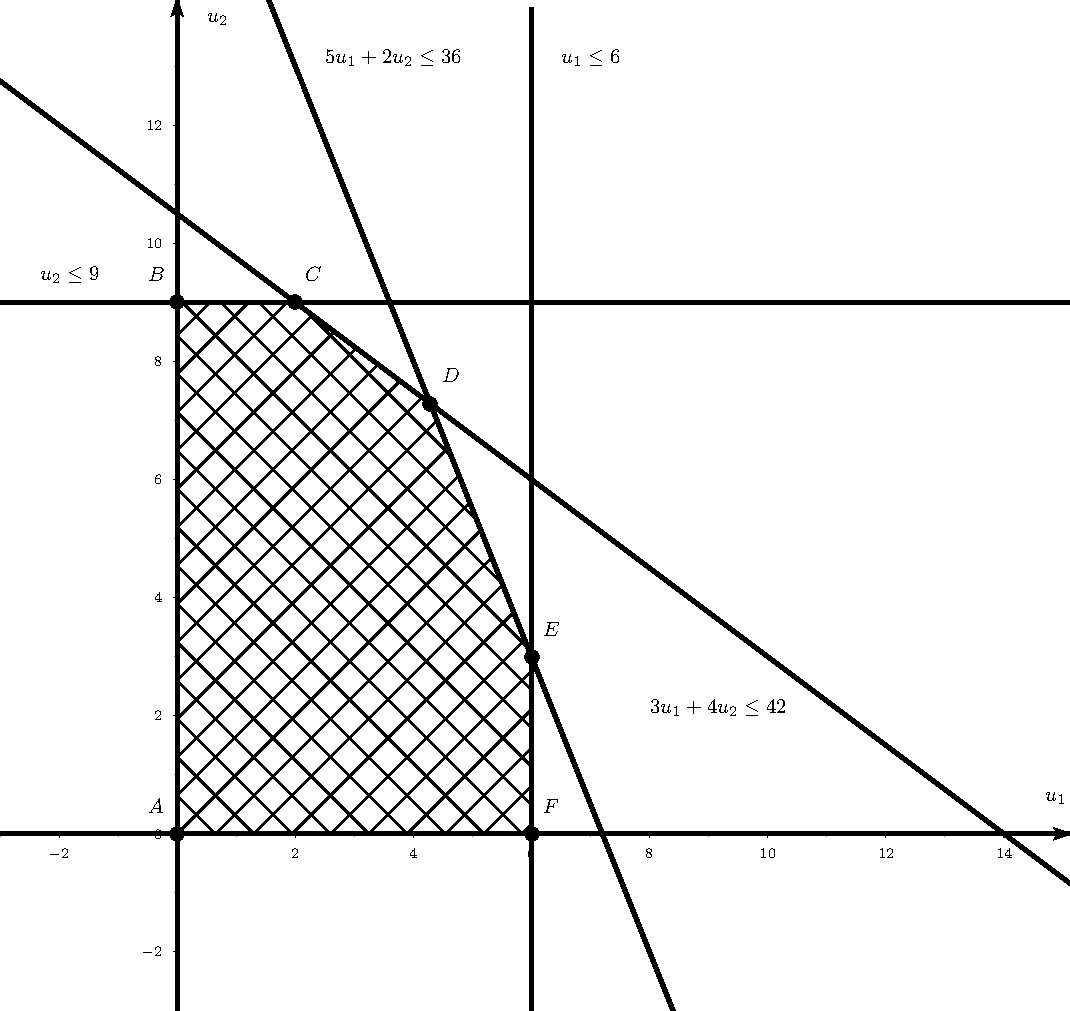
\includegraphics[scale=0.7]{img/dualSol.pdf} \\ 
	Solução ótima $u = (2,9)$
	\\ \ \\
	Encontrar solução ótima de (P) utilizando as relações das folgas complementares: \\ 
Das folgas complementares, se $x = (x_1, x_2,x_3,x_4)$ é viável no primal, $u = (u_1, u_2)$ é viável no dual e ambos satisfazem as equações:
	$$(c_j - u^TA_j) x_j = 0 \quad \forall j $$
	$$ u_i(a_{i}^Tx - b_i) = 0 \quad \forall i $$
	então $\overline{x}$ é ótimo no primal e $\overline{u}$ no dual. Tem que: 
	\begin{equation*}	
	\begin{array}{rcl}
	(u_1 - 6)x_1 & = & 0   \quad \Rightarrow  \quad  (2 - 6)x_1 = 0  \quad \Rightarrow  \quad  x_1 = 0\\
	(u_2 - 9)x_2 & = & 0  \quad \Rightarrow  \quad (9 - 9)x_2 = 0  \quad \Rightarrow  \quad x_2 =~?\\
	(3u_1 + 4u_2 - 42)x_3 & = & 0 \quad \Rightarrow  \quad (42 - 42)x_3 = 0 \quad \Rightarrow  \quad  x_3 =~?\\
	(5u_1 + 2u_2 - 36)x_4 & = & 0   \quad \Rightarrow  \quad   (28 - 36)x_4 = 0 \quad \Rightarrow  \quad x_4 = 0 \\
	\end{array}
	\end{equation*}	
Tem-se que $x_1 = 0$ e $x_4 = 0$.
	\begin{equation*}	
	\begin{array}{rcl}
	 2(3x_3 + 5x_4 - 2) & = & 0  \quad \Rightarrow  \quad 3x_3 = 2  \Rightarrow x_3  = \frac{2}{3} \\
	9(x_2 + 4x_3 + 2x_4 - 3) & = & 0   \quad \Rightarrow  \quad x_2 + 4\times\frac{2}{3} - 3= 0  \Rightarrow  x_2 = \frac{1}{3} \\
	\end{array}
	\end{equation*}	
	Portanto, temos que
	$$z = 6\times 0 + 9 \times \frac{1}{3} + 42 \times \frac{2}{3} + 36 \times 0 = 31,$$
	o que confirma que $x_1 =0,~x_2=\frac{1}{3},~x_3=\frac{2}{3}~\text{e}~x_4=0$ é solução ótima de (P)
	\end{solution}
	

		

\question Seja
	\begin{equation*}
		  \begin{array}{crrrrrrrrrrcc}
 \text{(P):} & \text{Minimizar} & 2x_1 & + & 3x_2 & + & 5x_3 & + & 2x_4 & + & 3x_5 &      & \\   
  	   & \text{sujeito a:}&        &   &      &   & &  & & & & \\
  	   &                  &  x_1 & + &  x_2 & + & 2x_3 & + & x_4 & + & 3x_5   &  \geq & 4 \\
  	   &                &  2x_1 & - & 2x_2 & + & 3x_3 & + & x_4 & + & x_5  & \geq& 3\\
  	   &                 &   \multicolumn{11}{c}{x_i \geq 0,~ i=1,\dots,5.}      
		  \end{array}	
	\end{equation*}
%  	                   &     & x_j \geq 0,~j= 1,2,\ldots,5.&      &
	\begin{enumerate}[a)]	
		\item Escrever $(D)$ o problema dual de $(P)$. 
		\begin{solution}\\
	\begin{equation*}	
				\begin{array}{c r r c r c c }
			(D) :&  \text{Maximizar}   & 4u_1 & + & 3u_2 \\
			& \text{sujeito a:} & u_1    & + & 2u_2 & \leq   & 2 \\
			&                 & u_1    & -  & 2u_2 & \leq   & 3 \\
			&                 & 2 u_1 & + & 3u_2 & \leq  & 5 \\
			&                 & u_1    & +  &  u_2  & \leq   &  2 \\			
			&                 & 3u_1  & + &  u_2   & \leq   & 3 \\			
			&                 & \multicolumn{5}{c}{u_1,~u_2 \geq 0}
			\end{array}
	\end{equation*}

		\end{solution}		
		\item Resolver graficamente $(D)$. 
			\begin{solution}
				\begin{center}
					%\includegraphics[scale=.5]{dual.png}
				\end{center}
			A solução ótima do dual é $u^{\star} = (\frac{4}{5},\frac{3}{5})$, com valor de função objetivo $5$.
			\end{solution}
	\end{enumerate}

\section*{Dual Simplex}



\end{questions}

\end{document}
